\documentclass{article}
\usepackage{times}
\usepackage{tikz}
\usepackage{verbatim}
\usepackage{hyperref} 
\usepackage{graphicx}
\usepackage{natbib}
\usepackage{amsmath,amssymb}
\DeclareMathOperator*{\argmin}{arg\,min}
\DeclareMathOperator*{\sign}{sign}
\DeclareMathOperator*{\Lik}{Lik}
\DeclareMathOperator*{\Peaks}{Peaks}
\DeclareMathOperator*{\HotSpots}{HotSpots}
\newcommand{\Cost}{\text{Cost}}
\usepackage{stfloats}
\DeclareMathOperator*{\Diag}{Diag}
\DeclareMathOperator*{\TPR}{TPR}
\DeclareMathOperator*{\Segments}{Segments}
\DeclareMathOperator*{\FPR}{FPR}
\DeclareMathOperator*{\argmax}{arg\,max}
\DeclareMathOperator*{\maximize}{maximize}
\DeclareMathOperator*{\minimize}{minimize}
\newcommand{\ZZ}{\mathbb Z}
\newcommand{\NN}{\mathbb N}
\newcommand{\RR}{\mathbb R}

\usepackage{icml2015}

\icmltitlerunning{Learning penalties for peak detection in count data}

\begin{document}

\twocolumn[
\icmltitle{Learning penalties for peak detection in count data}

% It is OKAY to include author information, even for blind
% submissions: the style file will automatically remove it for you
% unless you've provided the [accepted] option to the icml2015
% package.
\icmlauthor{Guillem Rigaill}{rigaill@evry.inra.fr}
\icmladdress{INRA, Evry, France}
\icmlauthor{Toby Dylan Hocking}{toby.hocking@mail.mcgill.ca}
\icmlauthor{Guillaume Bourque}{guil.bourque@mcgill.ca}
\icmladdress{McGill genome center, Montreal, Quebec, Canada}

% You may provide any keywords that you 
% find helpful for describing your paper; these are used to populate 
% the "keywords" metadata in the PDF but will not be shown in the document
\icmlkeywords{segmentation, count data, penalty functions}

\vskip 0.3in
]

\begin{abstract}
  Peak detection is a central problem in ChIP-seq data analysis, and
  current algorithms for this task are unsupervised and mostly
  effective for a single data type (e.g. histone H3K4me3 profiles with
  sharp peaks). We propose PeakSeg, a supervised peak detection
  algorithm based on constrained optimal segmentation, which is easy
  to tune since it has only one free parameter: the optimal number of
  peaks. We propose to tune it using annotated regions in a supervised
  penalty function learning problem, which we show results in
  state-of-the-art peak detection for both sharp H3K4me3 and broad
  H3K36me3 data types. 
\end{abstract}

\section{Introduction to supervised ChIP-seq peak detection}

Chromatin immunoprecipitation sequencing (ChIP-seq) is a genome-wide
assay to profile histone modifications and transcription factor
binding sites, with many experimental and computational steps
\citep{practical}. Briefly, each experiment yields a set of sequence
reads which are aligned to a reference genome, and then the data are
interpreted by counting the number of aligned reads at each genomic
position. In this paper we propose a new method for peak calling these
data, which is a binary classification problem for each genomic
position. The positive class is enriched (peaks) and the negative
class is background noise.

More concretely, a ChIP-seq profile on a single
chromosome with $d$ base pairs is a vector $\mathbf y=
\left[
  \begin{array}{ccc}
    y_1 & \cdots & y_d
  \end{array}
\right]\in\ZZ_+^d$ of counts of aligned sequence reads. A peak
detection algorithm can be described as a function $c:\ZZ_+^d
\rightarrow \{0, 1\}^d$ which returns 0 for background noise and 1 for
a peak. In contrast to the supervised method proposed in this paper,
most previous algorithms are unsupervised since they define a peak
detector $c$ using only the profile data $\mathbf y$.

In supervised peak detection \citep{hocking2014visual}, there
are $n$ annotated samples, and each sample $i\in\{1, \dots, n\}$ has a
profile $\mathbf y_i\in\ZZ_+^d$ and a set of annotated regions $R_i$
which defines a non-convex annotation error function
\begin{equation}
  \label{eq:error}
  E[c(\mathbf y_i),  R_i] =
  \text{FP}[c(\mathbf y_i), R_i] +
  \text{FN}[c(\mathbf y_i), R_i].
\end{equation}
The annotation error counts the number of false positive (FP) and
false negative (FN) regions, so it takes values in the non-negative
integers. The goal is to find a peak caller with minimal error on some
test profiles:
\begin{equation}
  \label{eq:min_error}
  \minimize_c \sum_{i\in\text{test}} E[c(\mathbf y_i),  R_i].
\end{equation}

\textbf{TODO}: figure showing different patterns in different data sets.

\section{Related work}

In the benchmark data set of \citet{hocking2014visual}, there are two
different histone mark types: H3K4me3 (sharp peaks) and H3K36me3
(broadly enriched regions). The best peak detection algorithm for
these H3K4me3 data was macs \citep{MACS}, and the best for H3K36me3
was HMCan \citep{HMCan}. Both of these algorithms are unsupervised,
but were calibrated using the annotated region labels to choose the
best scalar significance threshold hyperparameter via grid search.

The ChIP-seq segmentation model we propose is a constrained version of
the Poisson model proposed by \citet{Segmentor}. Specifically,
they proposed to search all possible change-points to find the optimal
segmentation, but we propose to constrain the possible change-points to
the subset of models that can be interpreted as peaks.

\textbf{TODO}: discuss penalty functions \citep{cleynen2013segmentation}.

\section{From unconstrained to constrained maximum likelihoood
  segmentation}

In this section we discuss Poisson maximum likelihood segmentation
models for count data. First, we discuss an existing unconstrained
model, and then we propose a constraint that makes the model suitable
for peak detection.

\subsection{Unconstrained maximum likelihood segmentation}

\begin{figure*}[b!]
  \centering
  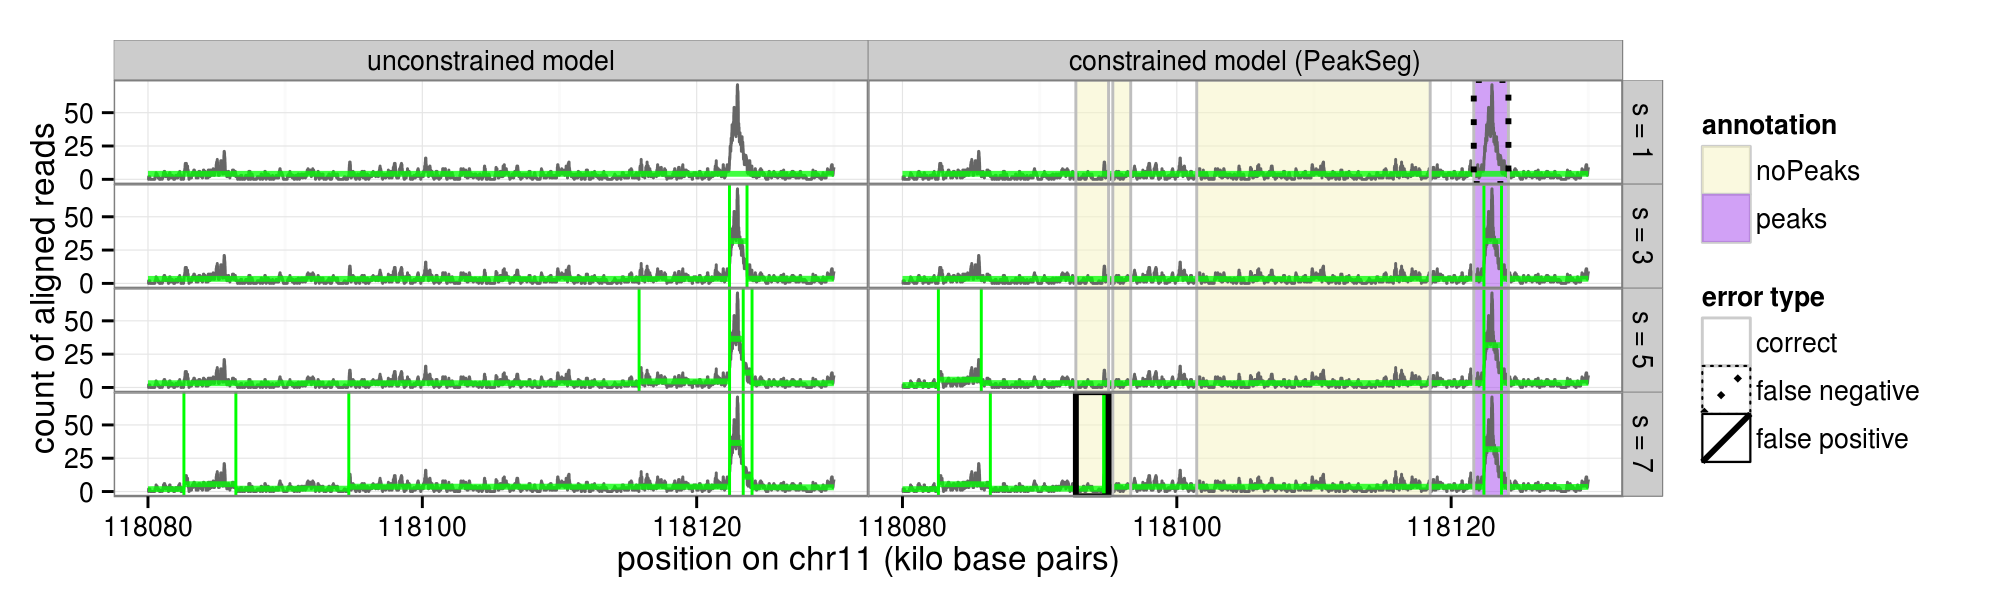
\includegraphics[width=\textwidth]{figure-Segmentor-PeakSeg}
  %\input{figure-Segmentor-PeakSeg}
  \vskip -0.5cm
  \caption{Example profile $\mathbf y$ (grey), with green horizontal
    lines for the segmentation mean $\mathbf m$, and green vertical
    lines to emphasize change-points. For this particular profile
    $\mathbf y$, the unconstrained and contrained models are
    equivalent $\mathbf{\hat m}^s(\mathbf y) = \mathbf{\tilde
      m}^s(\mathbf y)$ for $s\in\{1, 3\}$ segments but not for
    $s\in\{5, 7\}$. For the constrained models, the even numbered
    segments are interpreted as peaks (\ref{eq:peaks}), whose accuracy
    can be quantified using the annotations (\ref{eq:error}).}
  \label{fig:profiles}
\end{figure*}

After fixing a maximum number of segments $1 \leq s_{\text{max}}\leq d$,
the unconstrained maximum likelihood segmentation problem is defined
for any $s\in\{1, 2, \dots, s_{\max}\}$ as
\begin{equation}
  \label{argmin:unconstrained}
  \begin{aligned}
    \mathbf{\hat m}^s(\mathbf y)  =\ 
    &\argmin_{\mathbf m\in\RR^{d}} && 
    \rho
    (\mathbf m, \mathbf y) \\
    \\
    &\text{such that} && \Segments(\mathbf m)=s,
  \end{aligned}
\end{equation}
where the Poisson loss function is
\begin{equation}
  \rho(\mathbf m, \mathbf y)= \sum_{j=1}^d m_j - y_j \log m_j.
\end{equation} 
The model complexity is the number of piecewise constant segments
\begin{equation}
  \Segments(\mathbf m)=1+\sum_{j=2}^d I(m_j \neq m_{j-1}),
\end{equation}
where $I$ is the indicator function. 

Although it
is a non-convex optimization problem, the sequence of segmentations
$\mathbf{\hat m}^1(\mathbf y), \dots, \mathbf{\hat
  m}^{s_{\text{max}}}(\mathbf y)$ can be computed in $O(s_{\text{max}}
d^2)$ time using dynamic programming (DP) algorithms \citep{bellman},
or in $O(s_{\text{max}} d \log d)$ time using pruned DP
\citep{pruned-dp, Segmentor}.

We refer to (\ref{argmin:unconstrained}) as the unconstrained problem
since $\mathbf{\hat m}^s(\mathbf y)$ is the most likely segmentation
of all possible models with $s$ segments. Several unconstrained models
are shown on the left of Figure~\ref{fig:profiles}, and for example
the 2nd segment of the model with $s=3$ segments appears to capture
the peak in the data. 
% In general, we would like to use the 2nd, 4th,
% ... segments as peaks, and the 1st, 3rd, ... segments as
% background. 
To construct a peak detector $c$, first define the sign of the change
before base $j\in\{2, \dots, d\}$ as
\begin{equation}
  \label{eq:sign}
  S_j(\mathbf m) = \sign( m_{j} - m_{j-1} ),
\end{equation}
with $S_1(\mathbf m)=0$ by convention. Furthermore we define the peak
indicator at base $j\in\{1, \dots, d\}$ as
\begin{equation}
  \label{eq:peaks}
  P_j(\mathbf m) = \sum_{k=1}^j S_k(\mathbf m).
\end{equation}
Then we define a peak detector $c(\mathbf y) = \mathbf P\left[
  \mathbf{\tilde m}^s(\mathbf y) \right]\in\{0, 1\}^d$, where
\begin{equation}
  \mathbf
P[\mathbf m] = \left[\begin{array}{ccc} P_1(\mathbf m) & \cdots &
    P_d(\mathbf m)
\end{array}\right].
\end{equation}
\subsection{A constrained model for peak detection}

In general for the unconstrained model $P_j(\mathbf m)\in\ZZ$, which
is problematic since we want to use it as a peak detector with binary
outputs $P_j(\mathbf m)\in \{0, 1\}$. 

For example in Figure~\ref{fig:profiles} there is a position $j$ for
which $P_j\left[ \mathbf{\hat m}^5(\mathbf y) \right]=2$ (since the
mean changes up, up, down, down). 

Thus we constrain the peak indicator $P_j(\mathbf
m)\in\{0, 1\}$, which results
in the constrained problem
\begin{eqnarray}
  \label{argmin:constrained}
  \mathbf{\tilde m}^s(\mathbf y)  =
    \argmin_{\mathbf m\in\RR^{d}} && 
    \rho(\mathbf m, \mathbf y) \\
    \text{such that} && \Segments(\mathbf m)=s, \nonumber \\
     \forall j\in\{1, \dots, d\}, &&P_j(\mathbf m) \in\{0, 1\}.
     \nonumber
\end{eqnarray}
Another way to interpret the constrained problem
(\ref{argmin:constrained}) is that the sequence of changes in the
segment means $\mathbf m$ must begin with a positive change and then
alternate: up, down, up, down, ... (and not up, up, down). Thus the
even numbered segments (2nd, 4th, etc) may be interpreted as peaks,
and the odd numbered segments (1st, 3rd, etc) may be interpreted as
background. 

Figure~\ref{fig:profiles} shows a profile where the constraint is
necessary. In particular, it is clear that unconstrained models with
$s\in\{5, 7\}$ segments do not satisfy $P_j[\mathbf{\hat m}^s(\mathbf
y)]\in\{0, 1\}$ for all positions $j\in\{1,\dots, d\}$ (since they
both have up, up, down changes).

\section{Algorithms}

In this section we propose algorithms that can compute the Poisson
constrained optimal segmentation model. We first propose a constrained
dynamic programming algorithm that can be used to recover a sequence
of constrained maximum likelihood segmentations, $\mathbf{\tilde
  m}^1(\mathbf y), \dots, \mathbf{\tilde m}^{s_{\text{max}}}(\mathbf
y)$ (Section~\ref{sec:constrained-dp}). Then, we show how an existing
algorithm can be used to learn a penalty function for choosing the
number of segments $s\in\{1, \dots, s_{\text{max}}\}$
(Section~\ref{sec:supervised}).

\subsection{Constrained dynamic programming}
\label{sec:constrained-dp}

We propose to use dynamic programming to compute the sequence of
maximum likelihood models $\mathbf{\tilde m}^1(\mathbf y), \dots,
\mathbf{\tilde m}^{s_{\text{max}}}(\mathbf y)$ satisfying this up-down
constraint.

\textbf{TODO}: more detailed description of dynamic programming.

The algorithm is in $O(s_{\text{max}} d^2)$ time, where $d$ is the
number of data points, using the compression scheme proposed by
\citet{Segmentor}. A free/open-source R package implementing the
dynamic
programming is available at\\
\url{https://github.com/tdhock/PeakSegDP}

\textbf{TODO}: discussion of when the DP does not recover the optimal
solution. Maybe a figure? Maybe not. Maybe a discussion of how many
times it returned all 10 models in the real data sets.

\subsection{Supervised penalty learning for peak detection}
\label{sec:supervised}

\begin{table*}
  \centering
  \begin{tabular}{lllll}
    name & complexity & smoothing & parameters learned & learning algorithm \\
    \hline
    AIC/BIC.0 & $s$ & AIC=2, BIC=$\log d_i$ & none & unsupervised \\
    AIC/BIC.1 & $s$ & 
    $\beta$ & 
    $\beta\in\RR_+$ & grid search \\
    AIC/BIC.3 & $s$ & 
    $e^\beta d_i^{w_1} (\max \mathbf y_i)^{w_{2}}$ & 
    $\beta, w_1, w_{2}\in\RR$ & interval regression \\
    AIC/BIC.41 & $s$ & 
    $\exp(\beta + \mathbf w^\intercal \mathbf x_i)}$ & 
    $\beta\in\RR, \mathbf w\in\RR^{40}$ & 
    interval regression \\
    oracle.0 & $s\left(1 + 4\sqrt{1.1 + \log(d_i/s)}\right)^2$ &
    $\beta$ & none & unsupervised \\
    oracle.1 & $s\left(1 + 4\sqrt{1.1 + \log(d_i/s)}\right)^2$ &
    $\beta$ & $\beta\in\RR_+$ & grid search \\
    oracle.3 \textbf{TODO} & $s\left(1 + 4\sqrt{1.1 + \log(d_i/s)}\right)^2$ &
    $e^\beta d_i^{w_1} (\max \mathbf y_i)^{w_{2}}$ & 
    $\beta, w_1, w_{2}\in\RR$ & interval regression \\
    oracle.41 \textbf{TODO} & $s\left(1 + 4\sqrt{1.1 + \log(d_i/s)}\right)^2$ &
    $\exp(\beta + \mathbf w^\intercal \mathbf x_i)}$ & 
    $\beta\in\RR, \mathbf w\in\RR^{40}$ & 
    interval regression \\
    %AIC & $s$ & 2 & none & unsupervised \\
    %BIC & $s$ & $\log d_i$ & none & unsupervised \\
    %mBIC & \multicolumn{2}{c}{see \citet{mBIC}} & none & unsupervised\\
  \end{tabular}
  \caption{Penalty functions considered in this paper.}
  \label{tab:penalties}
\end{table*}

\begin{figure*}[b!]
  \centering
  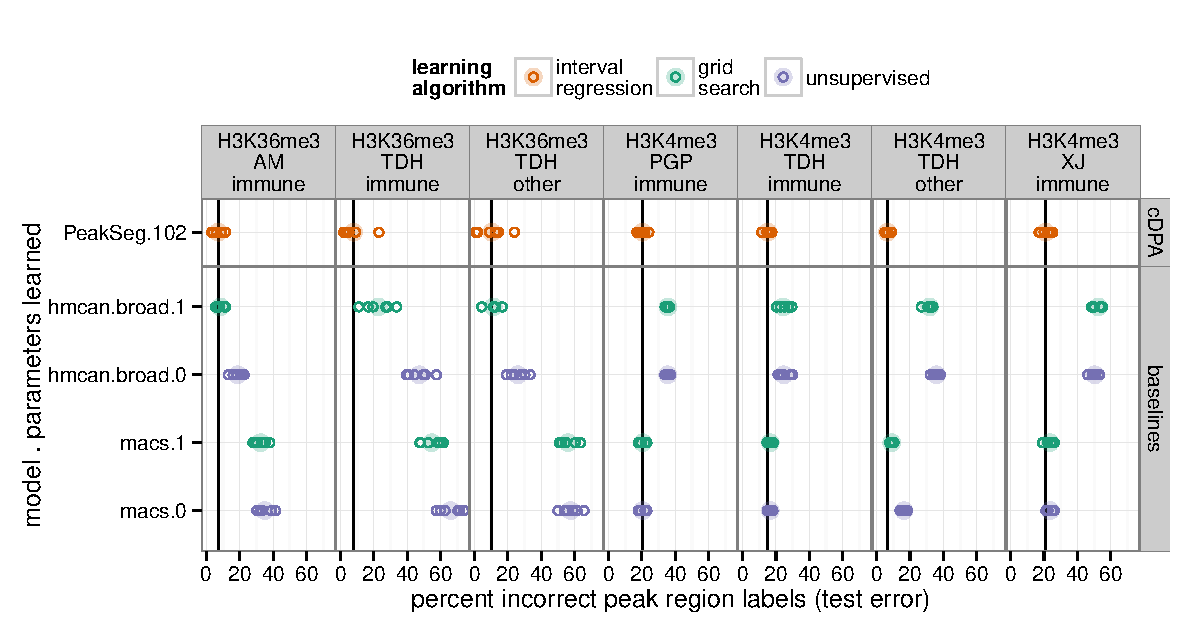
\includegraphics[width=\textwidth]{figure-dp-peaks-regression-dots}
  \vskip -0.5cm
  \caption{Test error of algorithms on seven annotated region data
    sets (each point shows one of six randomly selected train/test
    splits, and the shaded circle is the mean test error). Data set
    names show histone mark type (e.g. H3K36me3), annotator (AM), and
    cell types (immune). Colors show how the training data were used
    to learn model parameters parameters (grey ``cheating'' is not an
    algorithm but rather the best possible test error achievable by
    the constrained optimization models).}
  \label{fig:test-error}
\end{figure*}

After computing the constrained maximum likelihood segmentations for
each sample $i\in\{1,\dots, n\}$, the only question that remains is:
how many segments?

There are several existing penalty functions for resolving this model
selection problem. For example, one can use asymptotic arguments to
get a penalty such as the AIC (REF), BIC (REF), or mBIC (REF). More
recently, \citet{cleynen2013segmentation} proposed an oracle penalty
by applying finite sample model selection theory to segmentation
models of count data. All of these penalty functions are completely
unsupervised since they ignore the annotated region labels in the
training data set.

\citet{cleynen2013segmentation} proposed to use the 
un\-supervised heuristic of \citet{Lav05} for calibrating the penalty
constant $\beta$ in equation (6) of their paper. Instead, we propose to
use the annotated region labels as a super\-vised method for calibrating
this penalty constant $\beta$. More specifically, we defined a grid of
200 $\beta$ values evenly spaced on the log scale between $10^{-2}$
and $10^4$, then used grid search to select the value that minimizes
the annotation error (\ref{eq:error}) on the train set.

For supervised learning of multi-parameter linear penalty functions,
we can use the max margin interval regression algorithm of
\citet{HOCKING-penalties}. Briefly, we define the optimal number of
segments
\begin{equation}
  s^*(\lambda, \mathbf y) = 
  \argmin_{s\in\{1,3,\dots, s_{\text{max}}\}}
  \rho\left[
    \mathbf{\tilde m}^s(\mathbf y),
    \mathbf y
  \right]
  + \lambda s,
\end{equation}
where $\lambda\in\RR_+$ is a positive
penalty value. 

We define sample-specific features $\mathbf x_i\in\RR^m$ and penalty
values $\log \lambda_i = f(\mathbf x_i) = \beta + \mathbf w^\intercal
\mathbf x_i$, which is an affine function with parameters
$\beta\in\RR,\mathbf w\in\RR^m$ that will be learned. We considered
learning two models:

\begin{itemize}
\item \textbf{log.bases.log.max}: we used an $m=2$-dimensional feature
  vector $\mathbf x_i = \left[\begin{array}{cc} \log\max \mathbf y_i &
      \log d_i
\end{array}\right]$ where $d_i$ is the number of base pairs for 
sample/chromosome $i$.  This corresponds to a penalty $\lambda_i =
e^\beta (\max\mathbf y_i)^{w_1} d_i^{w_2}$. We trained the
model by solving problem (REF) with no regularization $\gamma=0$.
\item \textbf{L1.reg} we defined $m=41$ features using transforms ($x,
  \log x, \log[x+1], \log\log x$), where $x$ is: (un)weighted
  quartiles of $\mathbf y_i$, (un)weighted mean of $\mathbf y_i$, and
  number of (un)weighted data points $d_i$. We trained the model by solving
  problem (REF), using an internal cross-validation loop to estimate
  the regularization~$\gamma$.
\end{itemize}
The learning algorithm amounts to minimizing a
smooth convex loss $\ell_i:\RR\rightarrow\RR_+$ which depends on the
annotated region data $R_i$:
\begin{equation}
  \label{eq:relax}
  \hat f = \argmin_f \sum_{i=1}^n
  \ell_i\left[ f(\mathbf x_i) \right].
\end{equation}
Since $\ell_i$ is smooth and convex, this problem can be easily solved
using gradient-based algorithms. We used the accelerated gradient
method of the FISTA algorithm \citep{fista}.

To make a prediction on a
test sample with profile $\mathbf y$ and features $\mathbf x$, we
compute the predicted penalty $\hat \lambda = \exp \hat f(\mathbf x)$,
the predicted number of segments $\hat s = s^*(\hat \lambda, \mathbf
y)$, and finally the predicted peaks $\mathbf P\left[ \mathbf{\tilde
    m}^{\hat s}(\mathbf y) \right]$.

\section{Results: state-of-the-art peak detection for two data types}

We downloaded 7 benchmark data sets, which included a
total of 12,826 manually annotated regions\footnote{\url{http://cbio.ensmp.fr/~thocking/chip-seq-chunk-db/}}.
Since these genomic windows are relatively small, we set the maximum
number of segments $s_{\text{max}}=19$, and for each profile $\mathbf
y$ we computed $\mathbf{\tilde m}^1(\mathbf y), \dots, \mathbf{\tilde
  m}^{19}(\mathbf y)$ (\ref{argmin:constrained}). For the largest
profile we considered ($d=263,169$ weighted data points after
compression), the DP algorithm computed the 19 constrained optimal
segmentations in about 155 minutes.

We compared the proposed PeakSeg algorithm to the two previous
state-of-the-art peak detectors on this benchmark, macs and
\mbox{hmcan.broad}. For each data set, we randomly divided the
annotated windows into half train and half test. We trained the macs
and hmcan.broad algorithms by choosing the significance threshold with
minimal annotation error on the train set. We trained PeakSeg by
learning a penalty function $\hat f$ on the train set
(\ref{eq:relax}).

We show the percent test error for each algorithm and each data set in
Figure~\ref{fig:test-error}. As previously described
\citep{hocking2014visual}, macs had lower test error than
\mbox{hmcan.broad} for H3K4me3 data, and \mbox{hmcan.broad} had lower
test error than macs for H3K36me3 data. It is clear that our proposed
PeakSeg algorithm had lower test error than both macs and hmcan.broad
algorithms, for both data types.

\textbf{TODO}: discussion of unsupervised vs 1-parameter vs multi-parameter
learning.

% \begin{center}
%   \input{table-dp-peaks-regression}
% \end{center}

\section{Discussion, conclusions, and future work}

\textbf{TODO}: discuss machine learning for recognizing different
patterns, versus using several different unsupervised algorithms for
specific data sets. E.g. car/face detector versus generic object
detector trained on various different data sets.

% \begin{figure*}[t!]
%   \centering
%   \includegraphics[width=\textwidth]{figure-regularized-all}
%   \vskip -0.5cm
%   \caption{Normalized weights of the 2-feature log.bases.log.max model
%     compared to the 41-feature L1.reg model. In some data sets the
%     L1.reg model sets these feature weights to 0.}
%   \label{fig:regularized-all}
% \end{figure*}

% \begin{figure*}[t!]
%   \centering
%   \includegraphics[width=\textwidth]{figure-regularized-feature-importance}
%   \vskip -0.5cm
%   \caption{Importance of features in L1.reg models. There were several
%     features in H3K4me3 data sets which were selected in all 6
%     train/test splits (note that unweighted.quartile.100\% is the same
%     as the maximum of the data). For other data sets it is not clear
%     which features are most important.}
%   \label{fig:regularized-feature-importance}
% \end{figure*}

We proposed to use the solution of a constrained optimal segmentation
problem (\ref{argmin:constrained}) as a ChIP-seq peak detector. For
$d$ data points and $s_{\text{max}}$ segments, we proposed to use
dynamic programming to compute the solutions in $O(s_{\text{max}} d^2)$
time. Furthermore, we proposed to use annotated region data as
supervision in a penalty learning problem (\ref{eq:relax}). This
approach yields state-of-the-art test error rates for peak detection
in a benchmark that includes both H3K4me3 and H3K36me3 data
sets.

Although it has been previously proposed to train a peak detector
using a set of positive control peak regions \citep{DFilter}, PeakSeg
is the first algorithm that can be trained with both positive and
negative control regions. PeakSeg is also the first algorithm to
exhibit state-of-the-art accuracy on both sharp H3K4me3 and broad
H3K36me3 ChIP-seq profiles in the benchmark of
\citet{hocking2014visual}. In the future, even better accuracy may be
obtained by engineering better features $\mathbf x_i$ for the penalty
learning problem (\ref{eq:relax}), perhaps based on Poisson
segmentation model selection theory \citep{cleynen2013segmentation}.

The current implementation of PeakSeg using dynamic programming has
one major limitation. The $O(s_{\text{max}} d^2)$ time complexity has
limited its application to subsets of chromosomes of up to $d=263,169$
data points. In comparison, the largest chromosome in hg19 (chr1) has
$d=249,250,621$ base pairs. To apply PeakSeg to larger data sets, we
are investigating a constrained version of pruned dynamic programming
\citep{pruned-dp, Segmentor}, which has $O(s_{\text{max}} d\log d)$
time complexity.

Finally, we are interested in segmenting multiple samples $i$ at the
same time, since peaks are often observed in the same genomic location
across several samples of the same cell type. This joint peak
detection problem may lead to more accurate peak calls, but it is a
considerably more difficult segmentation problem.

\begin{table*}[b!]
  \centering
  \begin{tabular}{ccc}
    \textbf{learning algorithm} & \textbf{heuristics} & 
    \textbf{constrained optimization} \\
    \hline
    unsupervised & hmcan.broad.0, macs.0 & AIC/BIC.0, oracle.0 \\
    grid search & hmcan.broad.1, macs.1 & AIC/BIC.1, oracle.1 \\
    interval regression & --- & AIC/BIC.3, oracle.3 \\
    regularized interval regression & --- & AIC/BIC.41, oracle.41 \\
  \end{tabular}
  \caption{Comparison of peak detection methods for ChIP-seq data. 
    The two main contributions of this paper 
    are to show that peak detection can be improved 
    using constrained optimization and 
    interval regression to learn a 
    multi-parameter penalty function.}
  \label{tab:supervised-maxlik}
\end{table*}

\bibliographystyle{abbrvnat}

\bibliography{refs}

\end{document}
